\chapter{Modeling in biology} \label{ch:models}

In biology, ordinary differential equations (ODE:s) are a common tool for modeling systems mathematically.
The systems are modeled to contain several interacting species, and observable states of the different species.
The states vary from field to field, but common types are the concentration of a chemical species in biochemistry, the volume of organs or growths in medical science and the size of populations of certain animal species in ecology.
The interaction of the different species is modeled over time, and thus differential equations are a suitable tool.
The restriction to ODE:s is often due to the fact that the models required to describe biological phenomena are complex enough, without taking spaciality into account, to be at the boundaries of what is viable to simulate and compare to experiments.
There is therefore a large amount of models in these fields that take the form
\begin{align*}
  \begin{split} %\label{eq:generic-bio-ode}
    \diff{A^1}{t} &= \omega^1(t, A^1, \dots, A^s; \vect{\theta}) \\
    &\equalsvdots \\
    \diff{A^s}{t} &= \omega^s(t, A^1, \dots, A^s; \vect{\theta}),
  \end{split}
\end{align*}
where \(A^1(t), \dots, A^s(t)\) are the states at time \(t\), and \(\vect{\theta} = \left(\theta^1, \dots, \theta^m\right)\) are a collection of parameters.
The parameters allow the models to be adopted to a vast variety of circumstances.
They can be related to environmental factors, inherent properties of the species involved or a measurement of a species assumed to be constant for the duration of the experiment.

One major obstacle in modeling and predicting the behavior of biological systems is the ability to correctly estimate these parameters.
The reliance on estimated values in models is not unique to biology in the natural sciences, but unlike most other natural sciences the models in many biological fields are are constructed based on these types of experiments.
While one can in physics isolate different parts of a larger system, and part by part build a theoretical model that is then tested on larger systems, the same approach can not be used in biology as the systems studied are large and intertwined enough that isolation of phenomena becomes nigh on impossible.
Instead chemical principles, research on simpler but similar lifeforms and biological intuition is used to build models, which can then be tested against data from living test subjects (in vitro or in vivo).
Not only does this affect the speed at which good models can be constructed; it also means that the parameters values that can not be directly measured can not be estimated before any simulation of the model is run, since there is no underlying fundamental model to predict the values with.

To solve these problems, a number of advanced methods with have been developed with such sophistication that entirely new fields, such as systems biology, have developed around them \cite{kitano2002systems,westerhoff2004evolution}.
Still, many problems and challenges remain.
In this thesis, mathematical symmetries is explored as a possible tool to solve some of these challenges.
In order to tackle such a broad question as \enquote{Can symmetries be used to enhance biological modeling?}, several concrete models from biology have been selected as examples.
These examples serve both as a familiar setting for those working in biological modeling to learn about symmetries of differential equations, and as a way to concretely discuss the uses of these symmetries as modeling tools.

The models have been selected to cover a range of biological disciplines, and to cover model complexity ranging from models simple enough to solve by hand to those used in current research.
In this chapter the models will be introduced, along with some biological context where necessary.

\section{The Hill equation}

The Hill equation is a scalar ODE that was originally used to model the binding of oxygen to hemoglobin \cite{hill1913combinations}.
Since then, it has been used to describe many binding phenomena such as ligand--receptor and substrate-enzyme reactions \cite{weiss1997hill}.
It takes the form
\begin{equation} \label{eq:original-hill}
  \diff{Y}{t} = - v_\text{max} \frac{Y^n}{K_m + Y^n} = \Omega_n(t, Y), \quad
  n > 0,
\end{equation}
where \(Y\) is the concentration of the substrate that binds to the enzyme.
The parameter \(v_\text{max}\) models the maximum reaction speed, \(K_m\) is a dissociation constant and \(n\) is the Hill coefficient.
The biological interpretation of the Hill coefficient \(n\) has historically been a contentious matter, but it is roughly a measure of the cooperativity among binding sites.
The Hill equation has been studied using symmetries of differential equations, using its nondimensionalized form \cite{ohlsson2020symmetry}.
By nondimensionalizing both the substrate concentration with
\begin{equation*}
  y = \frac{Y}{{K_m}^{1/n}}
\end{equation*}
and the time with
\begin{equation*}
  \tau = v_\text{max} \frac{t}{{K_m}^{1/n}},
\end{equation*}
\cref{eq:original-hill} simplifies to its nondimensionalized form
\begin{equation} \label[ode]{eq:hill}
  \diff{y}{\tau} = - \frac{y^n}{1 + y^n} = \omega_n(\tau, y), \quad
  n > 0
\end{equation}
which will be studied in this thesis.
% TODO: Plot

\section{The Gompertz model}

In several fields in- and outside of the life sciences, growth in general plays an important role.
In particular, when measuring different phenomena ranging from cell growth to the growth of cities, the concept of exponential growth often appears.
Exponential growth stems from a species growing with a rate that is proportional to its size.
Written in mathematical terms:
\begin{equation} \label{eq:exponential}
  \diff{W}{t} = c W(t),
\end{equation}
where \(W(t)\) is the size of the species (volume of a tumor, weight of an animal, individuals in a population etc.) at time \(t\) and \(c\) is a constant.
While exponential growth accurately models the initial stages of the growth process for many systems, eventually some external factor will limit the growth.
The external factor might be simple, like limited availability of food in the case of an animal population, or complex, like limitations of infrastructure in the case of cities. % FIXME: Check validity of statement
Correctly modeling the external limitations is crucial when studying the long term behavior of the system.

The Gompertz model is one such model that has seen success in many areas.
It was first proposed in 1825 as a means of predicting the mortality rate of populations in order to accurately prize life insurances and annuities \cite{gompertz1825nature}.
Gompertz formulated his model as the differential equation
\begin{equation} \label[ode]{eq:original-gompertz-modern}
  \diff{L}{x} = -a q^x L(x)
\end{equation}
where \(L(x)\) is the number of people living at age \(x\). % TODO: What is a and q?
It is worth noting that for small values of \(x\) and \(c = -a\), \cref{eq:original-gompertz-modern} behaves like \cref{eq:exponential}.
In retrospect this similarity is not surprising as Gompertz modeled the decay of a population, which can be seen as \enquote{negative growth}.
However, this connection was not made at first.

Around a hundred years after the conception of the model, it saw its first use as a growth model in the modeling of economic growth \cite{prescott1922demand,peabody1924railway}.
It was first mentioned in the life sciences in 1926 as a suggestion for an alternative growth model \cite{wright1926reviews}, and a few years later saw its first concrete use modeling the weight of cattle \cite{davidson1928growth}.
In the century since, the Gompertz model has been used to model the size of a wide range of animals (for a good summary, see \cite{tjorve2017gompertz}).
The breadth of animals (and parts of animals) where the Gompertz model can be fitted well to growth data has made this one of the life sciences where the model is most used.
The other branch of the life sciences where the Gompertz model has seen success is in modeling tumor growth.
The model was first used (apart from as a tool for making graphs \cite{casey1934alteration}) for this purpose in 1964 \cite{laird1964dynamics}.
It has since become one of the most widely used models for tumor growth \cite{gerlee2013muddle} (for a summary of applications, see the introduction of \cite{benzekry2014classical}).
When studying both organism and tumor growth, the same question have been asked about the Gompertz model, namely what the biological interpretation of the model is.
In this chapter, this question will be tackled using the theory of Lie point symmetries.

\subsection{Finding a standardized ODE description}

Even though Gompertz first stated his model as \cref{eq:original-gompertz}, the differential form is not the most commonly used.
Instead the Gompertz model is usually formulated as the solution to \cref{eq:original-gompertz-modern}.
In Gompertz' original paper \cite{gompertz1825nature}, this function takes the form
\begin{equation} \label{eq:original-gompertz-solution}
  L(x) = d g^{q^x}
\end{equation}
where \(g = \exp(-a/\ln\left(q\right))\) in \cref{eq:original-gompertz-modern}.
Note that the parameter \(d\) is not included in the differential equation but instead stems from the constant of integration.
By replacing Gompertz' \(L(x)\) (number of people of age \(x\)) with \(W(t)\) (the size of a species at time \(t\)) the function can be used to model growth without any structural changes to the function.
The function form of the model is not only sufficient as description when the goal is to fit the model to some data; the third parameter \(d\) is necessary since it relates to the initial value needed to solve \cref{eq:original-gompertz-modern}.
However, as will be seen in the next chapter, \cref{eq:original-gompertz-solution} is not a form where the type of symmetries used in this thesis can be employed.
Additionally, the function is not parametrized consistently across literature, varying depending on field and taste.
To analyze the model with Lie point symmetries it is therefore necessary to determine two things.
Firstly it must be established what is meant by \enquote{The Gompertz Model} when viewing the model as an ODE through a life since lens.
Secondly, a standardized and meaningful parametrization of the model in ODE form must be established in order to gain insight from the later symmetry treatment.

Since the function form of the model is sufficient and necessary to match the model to data, the ODE form is only found in the literature as a means of providing a background to the model.
The ODE formulation thus often lacks proper references, rendering the origin of the formulation hard to trace.
All formulations of the ODE found in the literature can however be sorted into one of three families.

The ODE:s in the first family can all be written on the form
\begin{equation} \label[ode]{eq:rough-gompertz-classical-ode}
  \diff{W}{t} = r e^{-b t} W(t).
\end{equation}
These ODE:s are reparameterizations of Gompertz' original ODE \labelcref{eq:original-gompertz-modern}, often emphasizing the expected behaviors of the model in the growth context by choosing parameters that should be positive.
In the parametrization seen in \cref{eq:rough-gompertz-classical-ode}, \(r\) should be positive for the species size \(W(t)\) to grow (as opposed to shrinking or decaying) and \(b\) should be positive for the growth to reduce over time (and thus limiting the growth).
Solutions to this family of ODE:s can be seen in \cref{fig:gompertz-classical-solutions}.

The first family of ODE:s is tightly related to the second family, which can be written on the form
\begin{equation}
  \label[ode]{eq:rough-gompertz-system-ode}
  \begin{aligned} 
    \diff{W}{t} &= G(t) W(t)\\
    \diff{G}{t} &= -b G(t).
  \end{aligned}
\end{equation}
This system of ODE:s could also be argued to be the original Gompertz ODE, since the original differential equation \labelcref{eq:original-gompertz-modern} was motivated by Gompertz in the following way:
\blockquote[{\cite[518]{gompertz1825nature}}]{
  If the average exhaustions of a man's power to avoid death were such that at the end of equal infinitely small intervals of time, he lost equal portions of his remaining power to oppose destruction which he had at the commencement of those intervals, then at the age his power to avoid death, or the intensity of his mortality might be denoted by \(aq^x\), \(a\) and \(q\) being constant quantities;
}
The intensity of mortality can be seen as \(\gamma(t)\) in \cref{eq:rough-gompertz-system-ode}, with \(\gamma(t) = aq^x\) serving as a solution to the lower equation in \cref{eq:rough-gompertz-system-ode} when \(\ln\left(q\right) = -b\).
Solutions to this family of ODE:s can be seen in \cref{fig:gompertz-system-solutions-varw,fig:gompertz-system-solutions-varg}.
Since \cref{eq:rough-gompertz-classical-ode} is a partial solution to \cref{eq:rough-gompertz-system-ode}, these two families of differential equations will henceforth be referred to collectively as \enquote{classical Gompertz ODE:s}, the latter formulation being specified as \enquote{classical Gompertz ODE:s on system form} or simply \enquote{system Gompertz ODE:s}.
The classical Gompertz ODE is the form used in the first paper on biological growth \cite{davidson1928growth}.
\begin{figure}
  \centering
  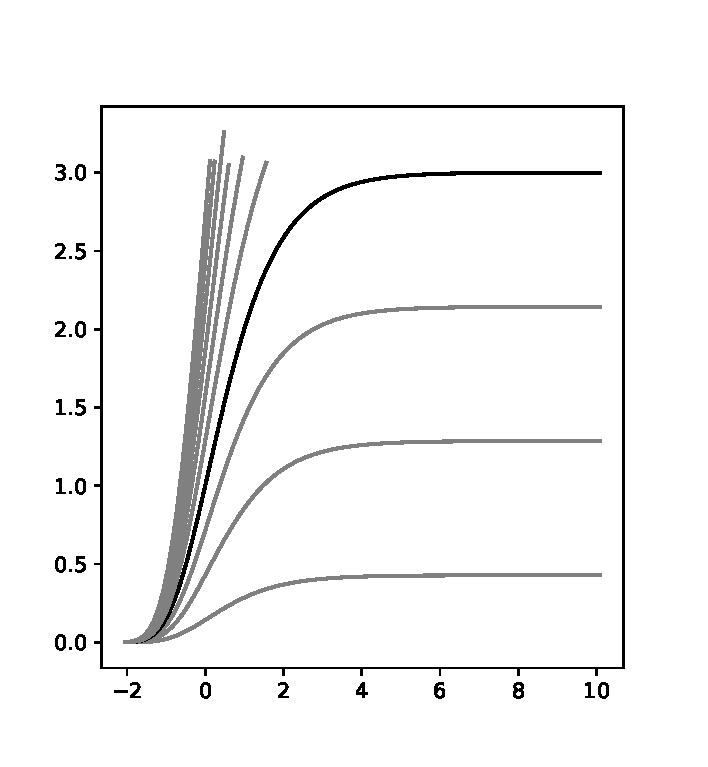
\includegraphics[width=.32\textwidth]{images/gompertz-classical-solutions}
  \caption{Example solutions curves of the classical Gompertz model with varying initial values for \(W\).}
  \label{fig:gompertz-classical-solutions}
\end{figure}
\begin{figure}
  \centering
  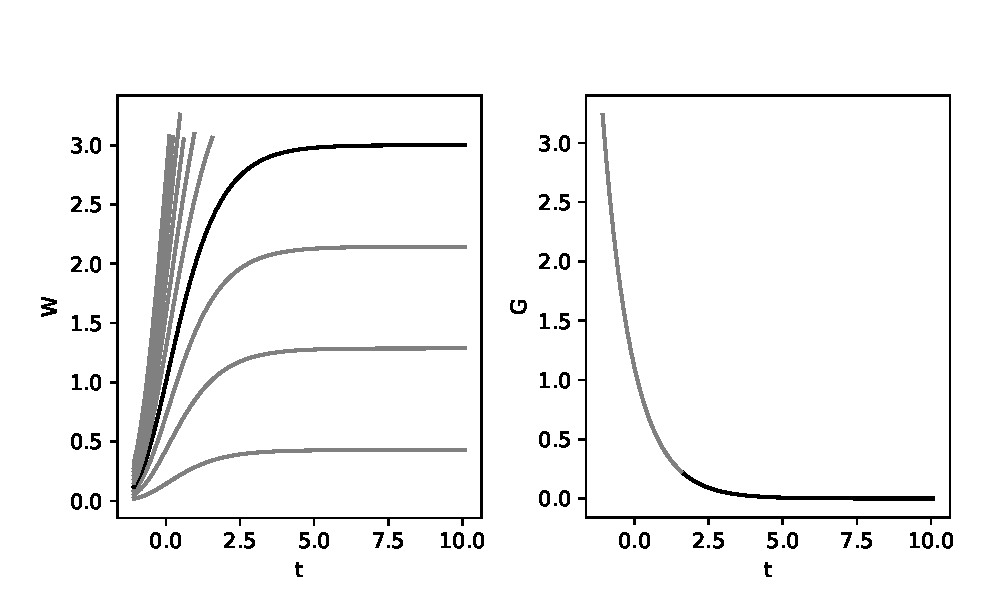
\includegraphics[width=.64\textwidth]{images/gompertz-system-solutions-varw}
  \caption{Example solutions curves of the system Gompertz model with varying initial values for \(W\).}
  \label{fig:gompertz-system-solutions-varw}
\end{figure}
\begin{figure}
  \centering
  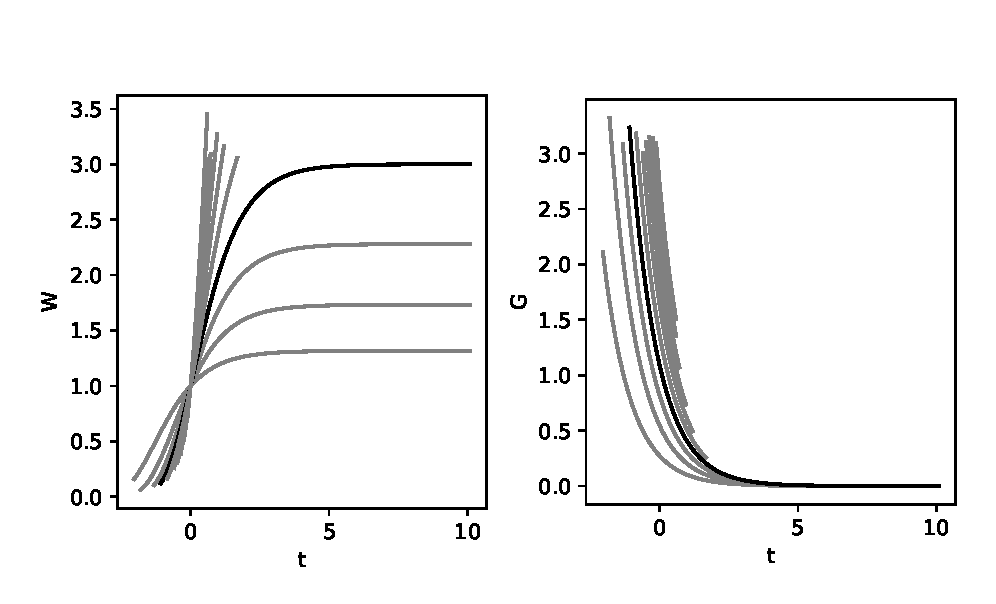
\includegraphics[width=.64\textwidth]{images/gompertz-system-solutions-varg}
  \caption{Example solutions curves of the system Gompertz model with varying initial values for \(G\).}
  \label{fig:gompertz-system-solutions-varg}
\end{figure}

The third family of ODE:s appear slightly later in the literature.
They can all be written on the form
\begin{equation} \label[ode]{eq:rough-gompertz-autonomous-ode}
  \diff{W}{t} = -\alpha \ln\left(\frac{W(t)}{K}\right) W(t).
\end{equation}
While solutions to this ODE are all Gompertz curves, it is important to note that this formulation is fundamentally different than the classical ODE \labelcref{eq:rough-gompertz-classical-ode}.
This is clear from the fact that while \cref{eq:rough-gompertz-classical-ode} is directly dependent on time, \cref{eq:rough-gompertz-autonomous-ode} is not.
We will therefore henceforth refer to the family of ODE:s that can be rewritten as \cref{eq:rough-gompertz-autonomous-ode} as \enquote{autonomous Gompertz ODE:s}.
Solutions to the autonomous Gompertz model can be seen in \cref{fig:gompertz-autonomous-solutions}
The first time an autonomous Gompertz ODE appears in the literature on biological growth is in a review of the new use of the Gompertz curve in 1932 \cite{winsor1932gompertz}.
In the review (which also features a classical Gompertz ODE) the autonomous form is used to liken the Gompertz curve to another popular growth curve, the logistic growth curve, in order to generalize the Gompertz model.
\begin{figure}
  \centering
  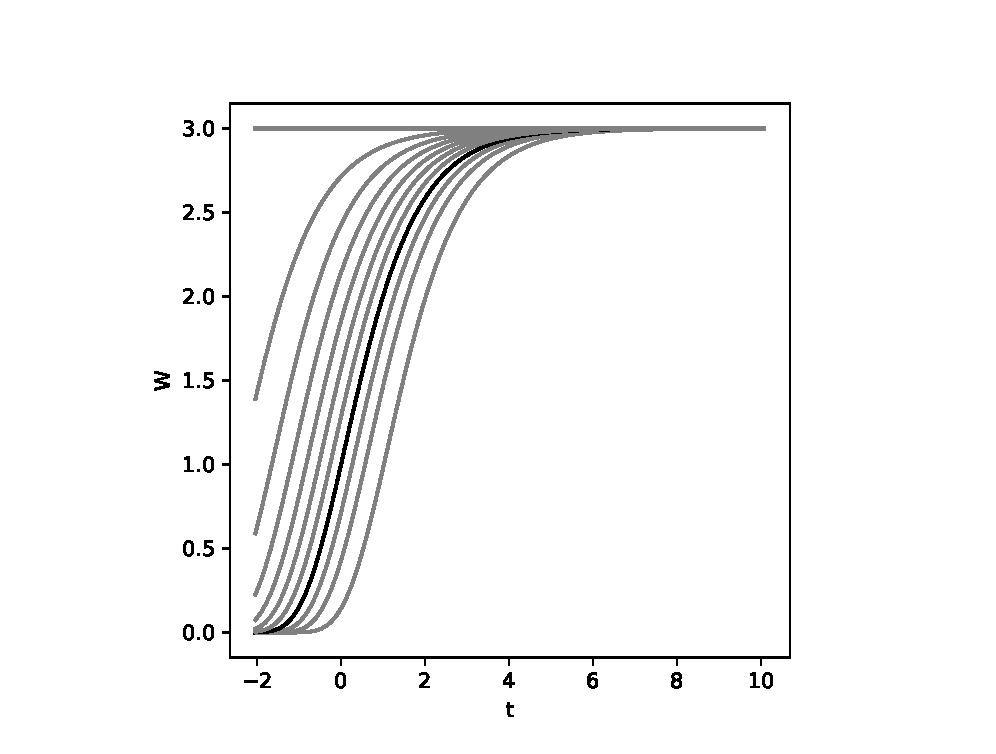
\includegraphics[width=.32\textwidth]{images/gompertz-autonomous-solutions}
  \caption{Example solutions curves of the autonomous Gompertz model with varying initial values for \(W\).}
  \label{fig:gompertz-autonomous-solutions}
\end{figure}

In order to better understand what separates the classical and autonomous ODE:s, a consistent parametrization is required.
Due to the sporadic use of the ODE form, no such standardization has been made.
The function form, on the other hand, has seen efforts of standardized parametrization.
\cite{tjorve2017gompertz} (concerned mainly with the growth of organisms) shows that most parametrizations found in the literature belong to two parametrization groups.
Both parametrizations groups have in common that they have two shape parameters and one location parameter, where this third parameter only controls how far the curve is shifted in the time direction.
In both groups the shape parameters serve the same purpose, but the location parameter can serve two distinct useful purposes, resulting in the two forms of parametrization: the \(T_i\)- and \(W_0\)-forms \cite{tjorve2017gompertz}.
These two forms can be canonically parametrized by
\begin{equation} \label{eq:gompertz-ti-function}
  W(t) = A e^{-e^{-k_G(t-T_i)}}
\end{equation}
and
\begin{equation} \label{eq:gompertz-w0-function}
  W(t) = A \left(\frac{W_0}{A}\right)^{-e^{-k_G t}}
\end{equation}
respectively.
These two parametrizations are useful, since the parameters \(A\), \(k_G\), \(T_i\) and \(W_0\) have clear interpretations. % TODO: Maybe plot this?
\(A\) is the value of the upper asymptote, also known as the carrying capacity of the system.
\(k_G\), although lacking in interpretation itself, is proportional to \(k_U = k_G / e\), where \(k_U\) is the relative (to \(A\)) maximum slope during the process.
Together, \(A\) and \(k_G\) control the shape of the curve.
\(T_i\) or \(W_0\) depending on the formulation control the localization of the curve.
\(T_i\) is the point in time where the curve achieves its maximum slope, also known as the point of inflection.
% TODO: Write about when this formulation is useful
\(W_0\) on the other hand is the size at \(t=0\).
Depending on application either of these two parametrizations might be useful.
It is therefore necessary to reparametrize both \cref{eq:rough-gompertz-classical-ode} and \cref{eq:rough-gompertz-autonomous-ode} using both forms.

To reparametrize the ODE:s using Gompertz curve parametrizations, the solutions of the ODE:s must be found.
The classical Gompertz ODE:s \labelcref{eq:rough-gompertz-classical-ode,eq:rough-gompertz-system-ode} are most easily solved using the fact that the classical ODE is separable to integrate over \(W\) and \(t\) separately.
The solutions are thus
\begin{equation} \label{eq:gompertz-classical-solution}
  W(t) = c e^{-r/b \cdot e^{-b t}}
\end{equation}
where \(c\) is an arbitrary constant.
The autonomous Gompertz ODE \labelcref{eq:rough-gompertz-autonomous-ode} is most easily solved using the variable substitution \(y(t) = \ln\left(W(t)/K\right)\) where the resulting ODE is readily solved.
The solutions are thus on the form
\begin{equation} \label{eq:gompertz-autonomous-solution}
  W(t) = K e^{c e^{-\alpha t}}
\end{equation}
where \(c\) is an integration constant.
Comparing the solutions in \cref{eq:gompertz-classical-solution,eq:gompertz-autonomous-solution} to the \(T_i\)- and \(W_0\)-formulations in \cref{eq:gompertz-ti-function,eq:gompertz-w0-function}, the relationships
\begin{align*}
  b &= k_G\\
  r &= k_G e^{k_G T_i}\\
  r &= k_G \ln\left(\frac{W_0}{A}\right)\\
  \alpha &= k_G\\
  K &= A
\end{align*}
between the parameters can be found.
The classical Gompertz ODE:s \labelcref{eq:rough-gompertz-classical-ode,eq:rough-gompertz-system-ode} and the autonomous Gompertz ODE \labelcref{eq:rough-gompertz-autonomous-ode} can thus be reparametrized as

\noindent
\begin{tabularx}{\linewidth}{rrM}
  Classical, & \(T_i\) :&
  \begin{minipage}{\linewidth}
    \begin{equation}
      \diff{W}{t} = k_G e^{-k_G (t - T_i)} W(t) \label{eq:gompertz-classical-ti}
    \end{equation}
  \end{minipage}\tabularnewline
  Classical, & \(W_0\) :&
  \begin{minipage}{\linewidth}
    \begin{equation}
      \diff{W}{t} = k_G \ln\left(\frac{W_0}{A}\right)e^{-k_G t} W(t) \label{eq:gompertz-classical-w0}
    \end{equation}
  \end{minipage}\tabularnewline
  Autonomous, & \(T_i\) and \(W_0\) :&
  \begin{minipage}{\linewidth}
    \begin{equation}
      \diff{W}{t} = -k_G \ln\left(\frac{W(t)}{A}\right) W(t) \label{eq:gompertz-autonomous}
    \end{equation}
  \end{minipage}\tabularnewline
  System, & \(T_i\) and \(W_0\) :&
  \begin{minipage}{\linewidth}%
    {\begin{subequations} \label[subequations]{eq:gompertz-system}
      \begin{align}
        \diff{W}{t} &= G(t) W(t) \label{eq:gompertz-system-a}\\
        \diff{G}{t} &= -k_G G(t). \label{eq:gompertz-system-b}
      \end{align}
    \end{subequations}}%
  \end{minipage}
\end{tabularx}
There are two important notes worth highlighting:
Firstly, all of the classical and autonomous formulations have a two-dimensional parameter space (even \cref{eq:gompertz-classical-w0} since \(W_0\) and \(A\) only appear in the composite form \(W_0 / A\)).
This must be the case since only a two parameter ODE can produce three parameter solutions (which the Gompertz curves are).
Secondly, it should be stressed that \cref{eq:gompertz-classical-ti,eq:gompertz-classical-w0} are just two different parametrizations of the same differential equation.
They will thus share symmetries, and calculations need only be performed on one form.


\section{The Lotka--Volterra predator--prey model}

A classic model for predator-prey dynamics is the Lotka--Volterra model, modeling two populations where one species feed on the other according to
\begin{subequations} \label[subequations]{eq:lotka-volterra}
  \begin{align}
    \diff{N}{t} &= a N - b N P\\
    \diff{P}{t} &= c N P - d P,
  \end{align}
\end{subequations}
where \(N\) is the prey population size and \(P\) the predator population size \cite{lotka1925elements,volterra1928variations}.
The parameter \(a\) the rate at which the prey population grows without interference, \(b\) and \(c\) how the predator and prey populations affect each other and \(d\) the rate at which predators die without prey to hunt.
Solutions to \cref{eq:lotka-volterra} can be seen in \cref{fig:lotka-volterra-solutions-varn,fig:lotka-volterra-solutions-varp}.
The Lotka--Volterra model is by no means the most modern or correct model to use in most situations, but the model is important from a historical perspective \cite{berryman1992orgins}.
Variations of the model have been analyzed using symmetries \cite{almeida1995lie,cherniha2004diffusive}, but there is a lack of interpretations of the symmetries in such literature as well as studies of the original model. % FIXME: Missing 2d-case with time invariance equivalent symmetry
\begin{figure}
  \centering
  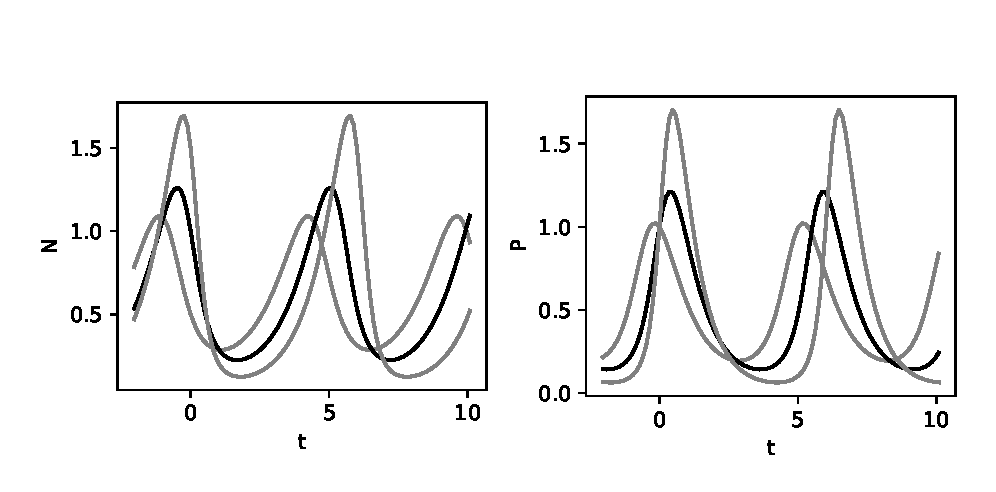
\includegraphics[width=.96\textwidth]{images/lotka-volterra-solutions-varn}
  \caption{Example solutions curves of the Lotka--Volterra predator--prey model with varying initial values for \(N\).}
  \label{fig:lotka-volterra-solutions-varn}
\end{figure}
\begin{figure}
  \centering
  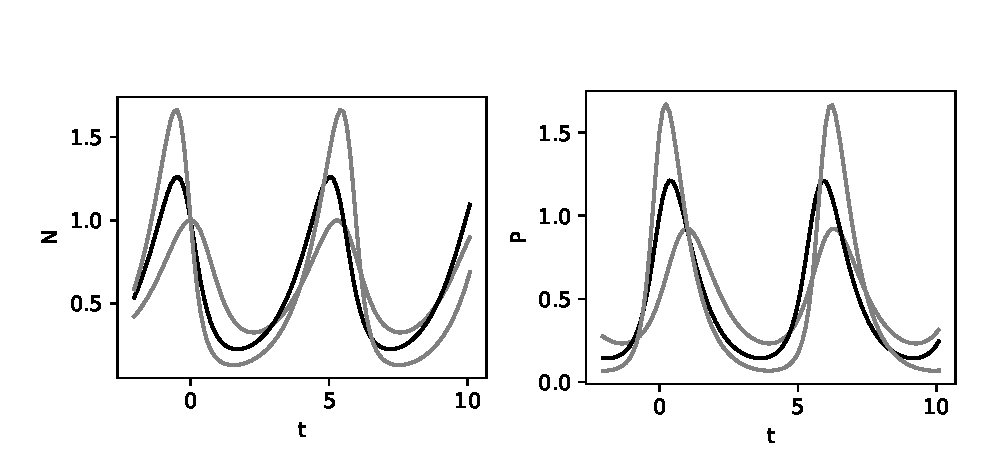
\includegraphics[width=.96\textwidth]{images/lotka-volterra-solutions-varp}
  \caption{Example solutions curves of the Lotka--Volterra predator--prey model with varying initial values for \(P\).}
  \label{fig:lotka-volterra-solutions-varp}
\end{figure}

\section{The Yildirim--Mackey lactose operon model}

A more modern model in the style and scope of those used today in biology is the Yildirim--Mackey model for the Lactose Operon \cite{yildirim2003feedback}.
It models the biochemical reaction to lactose in \textit{Escherichia coli} with a delay differential equation. % TODO: More description
Since this thesis only covers ODE:s, the slightly simplified ODE model used in \cite{yildirim2011deterministic} will instead be analyzed, which is modeled by
\begin{subequations} \label[subequations]{eq:lac-operon}
  \begin{align}
    \diff{M}{t} &= \alpha_M \frac{1 + K_1 A^n}{K + K_1 A^n} + \Gamma_0 - \gamma_M M \label{eq:lac-operon-a}\\
    \diff{B}{t} &= \alpha_B M - \gamma_B B \\
    \diff{L}{t} &= \alpha_L P \frac{L_e}{K_{L_e} + L_e} - \beta_{L_1} P \frac{L}{K_{L_1} + L} - \beta_{L_2} B \frac{L}{K_{L_2} + L} - \gamma_L L \\
    \diff{A}{t} &= \alpha_A B \frac{L}{K_L + L} - \beta_A B \frac{A}{K_A + A} - \gamma_A A \\
    \diff{P}{t} &= \alpha_P M - \gamma_P P,
  \end{align}
\end{subequations}
where \(M\) is mRNA production, \(B\) is the concentration of \(\beta\)-galactosidase, \(A\) is the concentration of allolactose, \(L\) is the concentration of intracellular lactose and \(P\) the concentration of permease. % TODO: Add quantities
